
\documentclass{beamer}

\usetheme{AnnArbor}
\usecolortheme{beaver}

\title{Censorship and Internet Engineering}
\author[Iain R. Learmonth]{Iain R. Learmonth \\ $<$irl@fsfe.org$>$ \\ 0x56FF9EA4E9846C49}
\institute[UoA / ORG]{University of Aberdeen / Open Rights Group}
\date{DRAFT}

\begin{document}

\begin{frame}
\maketitle
\end{frame}

\begin{frame}
	\frametitle{Hello}
	\begin{itemize}
		\item{University of Aberdeen's Electronics Research Group}
			\begin{itemize}
				\item{\url{http://www.erg.abdn.ac.uk/}}
			\end{itemize}
		\item{Open Rights Group}
			\begin{itemize}
				\item{\url{https://www.openrightsgroup.org/}}
			\end{itemize}
	\end{itemize}
\end{frame}

\begin{frame}
	\frametitle{Internet Measurements}
	\begin{itemize}
		\item{Measuring deployments}
		\item{Testing for path brokenness}
		\item{Real world environment}
	\end{itemize}
\end{frame}

\begin{frame}
	\frametitle{Enter Censorship}
	\begin{itemize}
		\item{The UK government has pressured ISPs to filter traffic to prevent children and young people from seeing content that is deemed unsuitable}
		\item{Results from blocked.org.uk (Top 100,000 websites\footnote{From the Alexa top 1 million websites}):}
		\begin{itemize}
			\item{TalkTalk Strict: 12982 blocked (13\%)}
			\item{Sky: 7006 blocked (7\%)}
			\item{TalkTalk Kidsafe: 5587 blocked (6\%)}
			\item{Virgin Media: 4320 blocked (4\%)}
		\end{itemize}
	\end{itemize}
\end{frame}

\begin{frame}
	\frametitle{The Lists}
	\begin{itemize}
		\item{Each ISP has a different block list}
		\item{Each ISP may even have many different block lists}
		\item{The lists are not publicly available}
	\end{itemize}
	\begin{center}
		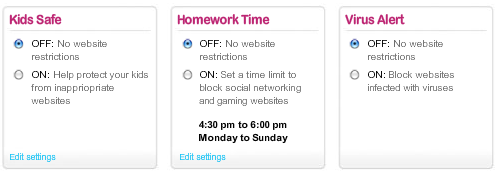
\includegraphics[width=0.7\textwidth]{talktalk.png}
	\end{center}
\end{frame}

\begin{frame}
	\frametitle{The Blocking}
	\begin{itemize}
		\item{Each ISP has a different way of dealing with requests for blocked content}
		\item{\url{blocked.org.uk} has complex rulesets for detecting blocked requests}
		\item{The blocks are not predictable}
	\end{itemize}
	\begin{center}
		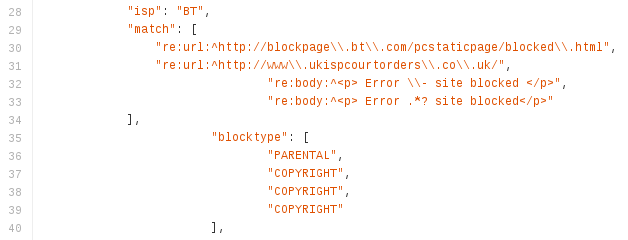
\includegraphics[width=0.7\textwidth]{blockedrules.png}
	\end{center}
\end{frame}

\begin{frame}
	\frametitle{Bad Science}
	\begin{itemize}
		\item{It's not possible to know easily when your experiment has
			been hijacked}
		\item{You end up measuring the ISP's filtering system and not
			the hosts you're really interested in}
	\end{itemize}
\end{frame}

\begin{frame}
	\frametitle{Solutions}
	\framesubtitle{HTTP 451 Unavailable For Legal Reasons}
	\begin{itemize}
		\item{draft-tbray-http-legally-restricted-status-05}
		\item{A new HTTP status code "for use when resource access is
			denied as a consequence of legal demands."}
		\item{Machine readable transparency}
	\end{itemize}
	\begin{center}
		
\includegraphics[width=0.7\textwidth]{http451.png}
	\end{center}

\end{frame}

\begin{frame}
	\frametitle{Solutions}
	\framesubtitle{HTTP 450 Blocked by Windows Parental Controls}
	\begin{itemize}
		\item{Used by Microsoft}
		\item{Can be generalised to cover all parental controls
			and age restricted content filters}
	\end{itemize}
	\begin{center}
		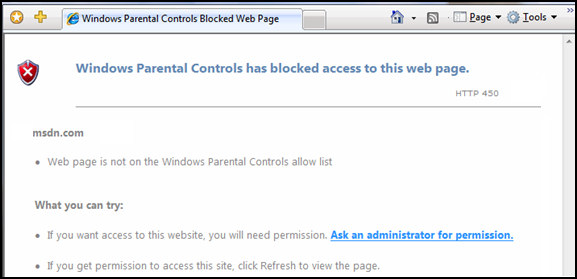
\includegraphics[width=0.7\textwidth]{http450.jpg}
	\end{center}
\end{frame}

\begin{frame}
	\frametitle{Solutions}
	\framesubtitle{More Transparency}
	\begin{itemize}
		\item{Online lookup tools}
	\end{itemize}
	\begin{center}
		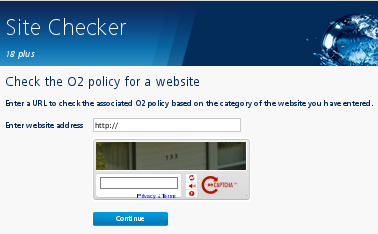
\includegraphics[width=0.7\textwidth]{o2checker.png}
	\end{center}
\end{frame}

\begin{frame}
	\frametitle{Thanks}
	\begin{center}
		{\LARGE Iain R. Learmonth $<$irl@fsfe.org$>$ \\ 0x56FF9EA4E9846C49}
		\ \\ \ \\
		{\LARGE \url{http://www.erg.abdn.ac.uk/}}
		{\LARGE \url{http://www.openrightsgroup.org/}}
		{\LARGE \url{http://www.blocked.org.uk/}}
	\end{center}
\end{frame}

\end{document}

